% ============================================================
% Capítulo 12: O Futuro da Engenharia de Software
% ============================================================
\chapter{O Futuro da Engenharia de Software}

\section{Introdução}

Prever o futuro é impossível. Preparar-se para ele é obrigatório.

\begin{itemize}
    \item \textbf{O que muda}: ferramentas, linguagens, paradigmas, velocidade de
    entrega, interfaces de interação com máquinas.
    \item \textbf{O que permanece}: a necessidade de resolver problemas reais para
    pessoas reais, com restrições reais de tempo, dinheiro e complexidade.
    \item \textbf{Tendências e sinais fracos}: o futuro não chega de uma vez. Ele se
    anuncia em papers de pesquisa, em demos que parecem brinquedo, em mudanças
    sutis no mercado de trabalho.
    \item \textbf{A armadilha da previsão}: em 2005, ninguém previu o iPhone. Em 2010,
    ninguém previu que deep learning resolveria visão computacional. Em 2020,
    ninguém previu o ChatGPT. O que não estamos prevendo agora?
    \item \textbf{A única constante}: a mudança em si. A velocidade da mudança está
    acelerando. A janela entre ``inovação de nicho'' e ``mainstream'' está
    encolhendo de décadas para meses.
    \item \textbf{Preparação sem previsão}: a estratégia não é adivinhar o futuro.
    É construir fundamentos sólidos o suficiente para se adaptar a qualquer
    cenário que venha.
\end{itemize}

Este capítulo final não pretende ser uma bola de cristal. É um exercício de
\textbf{pensamento estratégico} --- o mesmo tipo de pensamento que defendemos ao
longo de todo o livro, aplicado agora à nossa própria carreira e profissão.

\section{Evolução dos LLMs e Agents}

\subsection{Do GPT-3 aos Modelos Atuais: A Curva Exponencial}

Em 2020, o GPT-3 impressionou ao gerar texto coerente. Poucos imaginaram que, em
menos de cinco anos, modelos de linguagem estariam escrevendo código de produção,
arquitetando sistemas e colaborando em tempo real com engenheiros.

\begin{itemize}
    \item \textbf{GPT-3 (2020)}: 175 bilhões de parâmetros. Gerava código, mas
    frequentemente incorreto. Impressionava em demos, falhava em produção.
    \item \textbf{Codex e GitHub Copilot (2021)}: primeiro assistente de código
    amplamente adotado. Autocompletar com esteroides.
    \item \textbf{GPT-4 e Claude 3 (2023--2024)}: salto qualitativo em raciocínio.
    Capazes de entender contexto complexo, seguir instruções detalhadas,
    trabalhar com janelas de contexto de centenas de milhares de tokens.
    \item \textbf{Modelos de raciocínio (2024--2025)}: o1, Claude com pensamento
    estendido, Gemini. Capacidade de ``pensar antes de responder'', decompor
    problemas complexos, corrigir erros durante a geração.
    \item \textbf{Agents autônomos (2025--2026)}: modelos que não apenas respondem,
    mas \textbf{agem}. Executam comandos, navegam repositórios, criam PRs,
    iteram sobre feedback de testes.
\end{itemize}

\subsection{Agents Autônomos de Codificação}

Os coding agents representam uma mudança qualitativa na relação humano-IA.

\begin{itemize}
    \item \textbf{Claude Code}: agente de terminal que navega repositórios, edita
    arquivos, executa testes, corrige erros e itera até a solução funcionar.
    O engenheiro define o objetivo; o agente executa os passos.
    \item \textbf{Devin (Cognition)}: proposto como ``primeiro engenheiro de software
    IA''. Capaz de planejar, implementar e depurar de forma autônoma. Gerou
    enorme debate sobre o futuro da profissão.
    \item \textbf{OpenHands (ex-OpenDevin)}: alternativa open-source. Comunidade
    construindo agents de codificação transparentes e auditáveis.
    \item \textbf{Cursor, Windsurf, Copilot Workspace}: IDEs com IA integrada que
    borram a linha entre ``assistente'' e ``agente''.
    \item \textbf{O padrão emergente}: especificação em linguagem natural $\rightarrow$
    planejamento pelo agente $\rightarrow$ implementação iterativa $\rightarrow$
    validação por testes $\rightarrow$ revisão humana.
\end{itemize}

\subsection{Modelos Multimodais}

A fronteira da IA se expande para além do texto.

\begin{itemize}
    \item \textbf{Screenshot para código}: modelos que recebem uma imagem de interface
    e geram o código HTML/CSS/React correspondente. Precisão crescente.
    \item \textbf{Diagrama para implementação}: um diagrama de arquitetura se
    transforma em scaffolding de código, com serviços, APIs e banco de dados.
    \item \textbf{Voz para código}: descreva verbalmente o que quer; o modelo
    transcreve, interpreta e implementa.
    \item \textbf{Vídeo para testes}: grave a interação com o sistema; o modelo gera
    testes end-to-end automaticamente.
    \item \textbf{Implicação}: a barreira de entrada para criar software está
    diminuindo radicalmente. A barreira para criar \textit{bom} software permanece.
\end{itemize}

\subsection{Limites e Possibilidades}

\begin{itemize}
    \item \textbf{Scaling laws}: mais dados e mais computação melhoram os modelos, mas
    com retornos decrescentes. Não é crescimento infinito.
    \item \textbf{Alucinações}: problema fundamental da arquitetura de LLMs.
    Melhorando, mas dificilmente será eliminado por completo.
    \item \textbf{Raciocínio formal}: LLMs simulam raciocínio via padrões
    estatísticos. Provas formais e garantias matemáticas ainda são frágeis.
    \item \textbf{Custo computacional}: treinar e inferir modelos grandes consome
    energia equivalente a pequenas cidades. Sustentabilidade é uma barreira.
    \item \textbf{Dados de treinamento}: modelos são limitados pela qualidade e
    diversidade dos dados. Código legado e padrões ruins estão no treinamento
    tanto quanto boas práticas.
    \item \textbf{O teto de inteligência}: existe debate ativo sobre se LLMs podem
    alcançar raciocínio verdadeiramente geral ou se são otimizadores de
    padrões sofisticados. A resposta importa menos do que a utilidade prática.
\end{itemize}

\subsection{Timeline Realista vs. Hype}

O Gartner Hype Cycle oferece um modelo útil para entender onde estamos.

\begin{figure}[htbp]
    \centering
    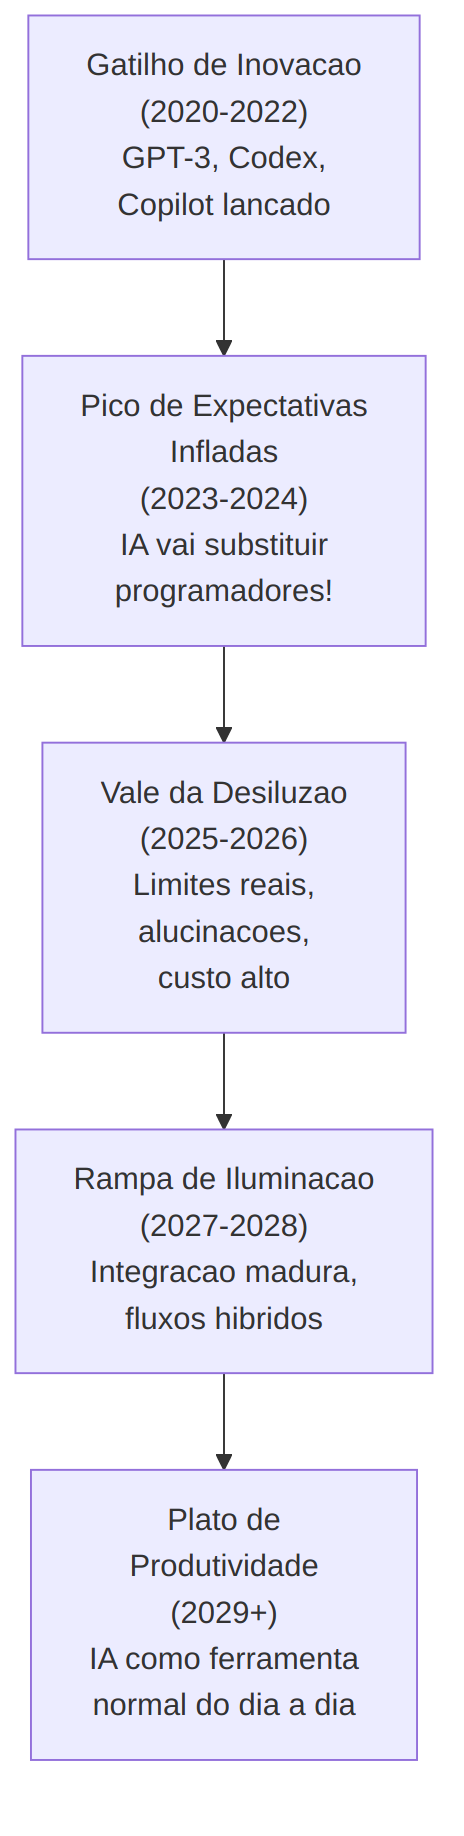
\includegraphics[width=0.85\textwidth]{imagens/12-futuro-engenharia-software-01-ciclo-de-hype-de-gartner-aplicado-a-ia-em-engenharia-de-soft.png}
    \caption{Ciclo de Hype de Gartner Aplicado à IA em Engenharia de Software}
\end{figure}

\begin{itemize}
    \item \textbf{Onde estamos (2026)}: entre o pico de expectativas infladas e o vale
    da desilusão. As promessas mais extremas não se concretizaram, mas o valor
    real é substancial.
    \item \textbf{O perigo do hype}: expectativas irreais levam a desilusão, que leva
    a abandono prematuro de tecnologias genuinamente úteis.
    \item \textbf{O perigo do ceticismo}: ignorar o potencial real da IA por causa
    das falhas atuais é tão perigoso quanto acreditar cegamente no hype.
    \item \textbf{Postura pragmática}: adotar o que funciona hoje, experimentar o que
    pode funcionar amanhã, ignorar o que é apenas marketing.
\end{itemize}

\section{O Engenheiro de Software em 2030}

\subsection{De Escritor de Código para Arquiteto de Sistemas}

O papel do engenheiro de software está em transformação acelerada.

\begin{figure}[htbp]
    \centering
    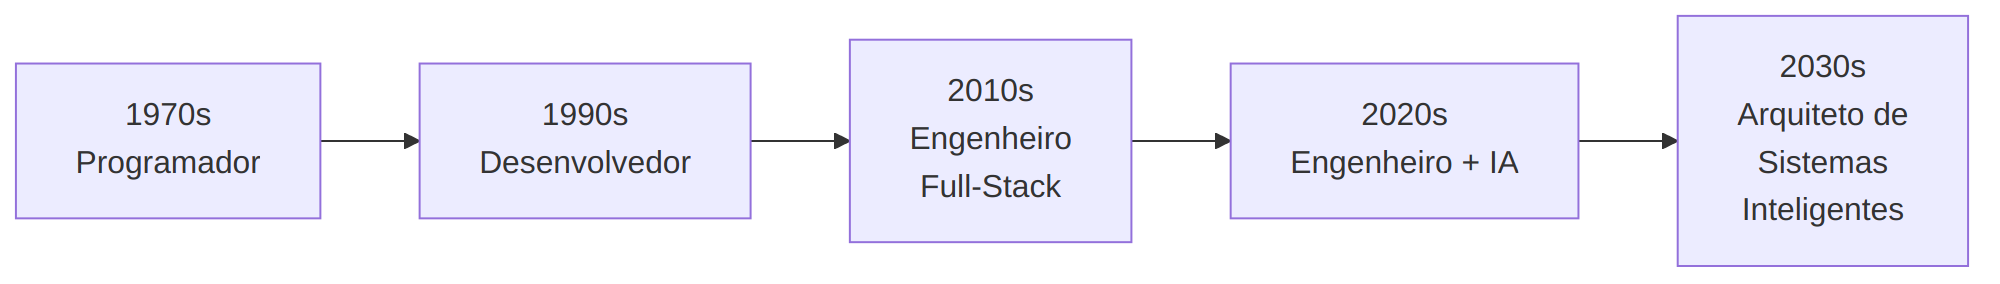
\includegraphics[width=0.85\textwidth]{imagens/12-futuro-engenharia-software-02-evolucao-do-papel-do-engenheiro-de-software.png}
    \caption{Evolução do Papel do Engenheiro de Software}
\end{figure}

\begin{itemize}
    \item \textbf{1970s --- Programador}: foco em traduzir algoritmos para linguagem de
    máquina. Domínio técnico puro.
    \item \textbf{1990s --- Desenvolvedor}: surge a internet, frameworks, bancos de dados
    relacionais. O desenvolvedor integra componentes.
    \item \textbf{2010s --- Engenheiro Full-Stack}: cloud, DevOps, microsserviços. O
    profissional opera do frontend ao deploy.
    \item \textbf{2020s --- Engenheiro + IA}: a IA entra como copiloto. O engenheiro
    orquestra humanos e máquinas.
    \item \textbf{2030s --- Arquiteto de Sistemas Inteligentes}: o engenheiro define
    a intenção, os constraints e os critérios de qualidade. Agents executam.
    O humano é o \textbf{cérebro estratégico}.
\end{itemize}

\subsection{Novas Habilidades Necessárias}

\begin{table}[h]
\centering
\caption{Habilidades do Engenheiro: Hoje vs. 2030}
\begin{tabular}{p{5.5cm} p{5.5cm}}
\toprule
\textbf{Hoje (2026)} & \textbf{2030+} \\
\midrule
Escrever código limpo & Especificar intenção com precisão \\
Debugar manualmente & Validar saídas de IA \\
Conhecer frameworks & Entender arquitetura de sistemas \\
Fazer deploys & Projetar pipelines autônomos \\
Escrever testes unitários & Definir critérios de aceitação para agents \\
Code review manual & Supervisão de código gerado por IA \\
Googlar soluções & Formular prompts eficazes \\
Dominar uma stack & Ser poliglota em paradigmas \\
Pair programming com humanos & Pair programming com IA \\
Ler documentação & Curar e filtrar informação \\
\bottomrule
\end{tabular}
\end{table}

\begin{itemize}
    \item \textbf{AI literacy}: entender como LLMs funcionam, suas limitações e seus
    vieses. Não precisa ser especialista em ML, mas precisa saber o que a
    ferramenta pode e não pode fazer.
    \item \textbf{Prompt engineering}: a capacidade de se comunicar precisamente com
    sistemas de IA. Não é moda passageira --- é a nova interface humano-máquina.
    \item \textbf{System design}: com a IA gerando código, o gargalo se move para
    decisões de arquitetura, trade-offs e design de alto nível.
    \item \textbf{Pensamento probabilístico}: IA não dá respostas certas --- dá
    respostas prováveis. O engenheiro precisa pensar em termos de confiança,
    não de certeza.
    \item \textbf{Curadoria e validação}: saber avaliar se o código gerado é correto,
    seguro, performático e adequado ao contexto.
\end{itemize}

\subsection{Especializações Emergentes}

\begin{itemize}
    \item \textbf{AI Engineer}: o profissional que constrói sistemas que usam IA.
    Diferente do ML Engineer (que treina modelos), o AI Engineer integra
    modelos em produtos.
    \item \textbf{Platform Engineer}: constrói a plataforma interna sobre a qual
    outros desenvolvedores trabalham. Infra como produto.
    \item \textbf{Developer Experience (DevEx) Engineer}: otimiza a experiência do
    desenvolvedor. Ferramentas, fluxos, documentação, onboarding.
    \item \textbf{Prompt Engineer / AI Interaction Designer}: projeta as interfaces
    de interação entre humanos e sistemas de IA.
    \item \textbf{Reliability Engineer evoluído}: de SRE para AIOps --- sistemas que
    se auto-monitoram e se auto-reparam.
    \item \textbf{Ethics Engineer}: profissional dedicado a garantir que sistemas
    de IA operam dentro de limites éticos e legais.
\end{itemize}

\subsection{O Que NÃO Vai Mudar}

\begin{itemize}
    \item \textbf{Pensamento crítico}: nenhuma IA substitui a capacidade de questionar
    premissas, identificar falácias e avaliar evidências.
    \item \textbf{Comunicação}: software é construído por equipes de humanos. Saber
    explicar, negociar e convencer continua essencial.
    \item \textbf{Conhecimento de domínio}: a IA não sabe que ``o cliente X tem uma
    cláusula contratual que proíbe cobrança dupla''. Contexto de negócio é
    humano.
    \item \textbf{Empatia}: entender o que o usuário realmente precisa (não o que ele
    pede) requer sensibilidade humana.
    \item \textbf{Responsabilidade}: quando o sistema falha, um humano responde. A IA
    não tem accountability.
    \item \textbf{Criatividade de alto nível}: combinar domínios, fazer analogias
    inesperadas, inventar categorias novas --- isso ainda é humano.
\end{itemize}

\subsection{O Efeito de Amplificação}

A IA não nivela. Ela amplifica.

\begin{itemize}
    \item \textbf{Engenheiros bons se tornam excelentes}: quem tem fundamentos sólidos
    usa a IA como um multiplicador. Pensa melhor, executa mais rápido, explora
    mais alternativas.
    \item \textbf{Engenheiros medianos se tornam substituíveis}: se a única habilidade
    é digitar código seguindo tutoriais, a IA faz isso mais rápido e mais barato.
    \item \textbf{A metáfora do amplificador}: um bom cantor com um microfone é
    magnífico. Um cantor ruim com um microfone é apenas mais alto.
    \item \textbf{Implicação prática}: investir em fundamentos (o tema deste livro)
    nunca foi tão importante.
\end{itemize}

\subsection{Desenvolvedores Juniores na Era da IA}

\begin{itemize}
    \item \textbf{O paradoxo}: juniores precisam praticar para aprender. Se a IA faz
    o trabalho ``fácil'', como eles aprendem?
    \item \textbf{O risco}: uma geração de desenvolvedores que sabe usar IA mas não
    entende o que ela gera. ``Engenheiros de prompt'' sem fundamentos.
    \item \textbf{A oportunidade}: a IA como tutor personalizado. Explica conceitos,
    gera exercícios, dá feedback imediato. Potencialmente o melhor professor
    que já existiu.
    \item \textbf{O caminho}: aprender \textit{com} a IA, não \textit{apesar} dela.
    Usar a IA para entender, não para evitar entender.
    \item \textbf{Recomendação}: alterne entre ``modo assistido'' (IA ligada) e
    ``modo solo'' (IA desligada). Construa fundamentos enquanto aproveita a
    produtividade.
\end{itemize}

\section{Novos Paradigmas de Desenvolvimento}

\subsection{Programação em Linguagem Natural}

\begin{itemize}
    \item \textbf{O conceito}: descrever o que o software deve fazer em português (ou
    inglês), e o sistema gera a implementação.
    \item \textbf{O estado atual}: funciona bem para tarefas bem definidas e isoladas.
    Falha em sistemas complexos com muitas dependências.
    \item \textbf{Spec-to-code}: a especificação detalhada em linguagem natural se
    torna o ``código fonte''. O código gerado é artefato, não autoria.
    \item \textbf{O problema}: linguagem natural é inerentemente ambígua. ``Rápido''
    significa 100ms ou 1s? ``Seguro'' significa autenticação ou criptografia
    end-to-end?
    \item \textbf{A convergência}: provavelmente teremos linguagens intermediárias
    entre o natural e o formal --- mais precisas que português, mais legíveis
    que Python.
\end{itemize}

\subsection{Programação Visual com IA}

\begin{itemize}
    \item \textbf{Diagramas executáveis}: desenhe um fluxograma e o sistema gera o
    código correspondente. O diagrama \textit{é} o programa.
    \item \textbf{Manipulação direta}: arraste componentes, conecte APIs, configure
    transformações. O código é gerado nos bastidores.
    \item \textbf{Limitação histórica}: programação visual sempre esbarrou na
    complexidade. Funciona para fluxos simples, colapsa em sistemas grandes.
    \item \textbf{O que muda com IA}: a IA pode preencher os ``gaps'' entre blocos
    visuais, gerando a lógica intermediária automaticamente.
\end{itemize}

\subsection{Low-Code/No-Code Evoluído}

\begin{itemize}
    \item \textbf{A evolução}: de plataformas limitadas e proprietárias para ambientes
    flexíveis assistidos por IA.
    \item \textbf{Citizen developers}: profissionais de negócio criando suas próprias
    ferramentas. O engenheiro de software como consultor e guardião.
    \item \textbf{O risco}: shadow IT em escala --- sistemas críticos construídos sem
    governança, segurança ou manutenibilidade.
    \item \textbf{O papel do engenheiro}: definir guardrails, templates, padrões
    de segurança. Não construir tudo, mas garantir que tudo seja construído
    direito.
\end{itemize}

\subsection{Programação por Exemplo}

\begin{itemize}
    \item \textbf{O conceito}: mostre ao sistema exemplos de entrada e saída desejada.
    Ele infere a transformação.
    \item \textbf{Já existe}: o ``Flash Fill'' do Excel é programação por exemplo.
    LLMs levam isso a outro nível de complexidade.
    \item \textbf{Limitação}: funciona para transformações de dados e padrões
    repetitivos. Não escala para lógica de negócio complexa.
\end{itemize}

\subsection{Desenvolvimento Baseado em Intenção}

\begin{itemize}
    \item \textbf{Intent-based development}: o engenheiro declara \textit{o que} quer
    (``o sistema deve processar 10.000 pedidos por segundo com latência abaixo
    de 200ms'') e o sistema determina \textit{como}.
    \item \textbf{Analogia}: é como Kubernetes para código. Você declara o estado
    desejado; o sistema se encarrega de atingi-lo.
    \item \textbf{Pré-requisito}: sistemas de teste e validação robustos o suficiente
    para verificar se a intenção foi cumprida.
    \item \textbf{Horizonte}: provavelmente 5--10 anos para maturidade em sistemas
    complexos. Já viável para domínios restritos.
\end{itemize}

\subsection{Onde Código Tradicional Ainda Vence}

\begin{itemize}
    \item \textbf{Sistemas críticos}: aviônica, dispositivos médicos, infraestrutura
    financeira. Onde cada linha precisa ser auditável e provável.
    \item \textbf{Performance extrema}: kernels, drivers, sistemas de tempo real.
    Controle bit-a-bit que IA generalista não oferece.
    \item \textbf{Algoritmos inovadores}: pesquisa de ponta em ciência da computação.
    A IA reproduz o conhecido; inovação requer criação original.
    \item \textbf{Código legado}: milhões de linhas de COBOL, Fortran e C que
    sustentam o mundo. Migração não é trivial nem urgente.
\end{itemize}

\subsection{O Problema da ``Última Milha''}

\begin{itemize}
    \item \textbf{O conceito}: a IA resolve 80\% do problema rapidamente. Os 20\%
    restantes --- edge cases, integrações, performance tuning --- tomam 80\%
    do tempo.
    \item \textbf{Analogia}: é como tradução automática. Funciona bem no geral, mas
    as nuances exigem um tradutor humano.
    \item \textbf{Implicação}: a IA não elimina a necessidade de engenheiros. Ela
    muda \textit{o que} eles fazem --- menos digitação, mais julgamento.
    \item \textbf{O valor do engenheiro}: está precisamente na última milha. É ali
    que se separa o software que funciona do software que funciona \textit{bem}.
\end{itemize}

\section{Ética e Impacto Social}

\subsection{Viés Algorítmico em Escala}

\begin{itemize}
    \item \textbf{O problema amplificado}: se um desenvolvedor tem viés, ele afeta
    seu código. Se um modelo de IA tem viés, ele afeta \textit{todo código
    gerado por ele}.
    \item \textbf{Exemplos reais}: sistemas de recrutamento que discriminam mulheres
    (Amazon, 2018), reconhecimento facial com taxas de erro muito maiores para
    pessoas negras (MIT, 2019), modelos de crédito que penalizam CEPs de
    bairros periféricos.
    \item \textbf{Viés nos dados de treinamento}: LLMs treinados em código existente
    herdam os vieses desse código --- padrões de naming, suposições culturais,
    prioridades de design.
    \item \textbf{Responsabilidade do engenheiro}: auditar, testar e questionar.
    ``A IA gerou'' não é desculpa para entregar software discriminatório.
\end{itemize}

\subsection{Impacto no Emprego}

A questão do emprego requer nuance, não pânico.

\begin{itemize}
    \item \textbf{O que a história ensina}: toda revolução tecnológica eliminou
    empregos E criou novos. O saldo líquido historicamente é positivo, mas a
    transição é dolorosa.
    \item \textbf{Empregos que diminuem}: codificação pura, trabalho repetitivo de
    manutenção, tarefas de integração simples.
    \item \textbf{Empregos que crescem}: AI engineering, system design, ética de IA,
    DevEx, curadoria de qualidade, consultoria de domínio.
    \item \textbf{O período de transição}: as próximas décadas terão deslocamento.
    Profissionais que se adaptam prosperarão. Os que resistem sofrerão.
    \item \textbf{Responsabilidade coletiva}: empresas, governos e comunidades técnicas
    têm o dever de facilitar a transição com requalificação e suporte.
    \item \textbf{Nuance geográfica}: o impacto é diferente no Vale do Silício,
    em São Paulo e em Manaus. Contexto local importa.
\end{itemize}

\subsection{Software e Sustentabilidade}

\begin{itemize}
    \item \textbf{Green computing}: datacenters consomem 1--2\% da eletricidade mundial.
    Treinar um único LLM grande emite centenas de toneladas de CO2.
    \item \textbf{Código eficiente como ato ambiental}: software otimizado consome
    menos CPU, menos memória, menos energia. Cada ciclo de clock economizado
    se multiplica por bilhões de execuções.
    \item \textbf{Sustentabilidade de IA}: o custo energético de inferência será
    uma preocupação crescente. Modelos menores e mais eficientes serão
    necessários.
    \item \textbf{O papel do engenheiro}: considerar impacto ambiental nas decisões
    de arquitetura. Cloud regions com energia renovável, algoritmos eficientes,
    cache inteligente.
\end{itemize}

\subsection{Regulação e Compliance}

\begin{itemize}
    \item \textbf{EU AI Act}: a regulação europeia classifica sistemas de IA por risco
    (inaceitável, alto, limitado, mínimo). Sistemas de alto risco exigem
    auditoria, transparência e supervisão humana.
    \item \textbf{LGPD e IA}: o uso de dados pessoais para treinar modelos está sob
    escrutínio. Consentimento, finalidade e minimização se aplicam.
    \item \textbf{Responsabilidade civil}: quando código gerado por IA causa dano,
    quem é responsável? O engenheiro, a empresa, o fornecedor do modelo?
    Legislação ainda está se formando.
    \item \textbf{Tendência global}: mais regulação, não menos. Engenheiros precisam
    entender compliance como parte do trabalho, não como obstáculo.
    \item \textbf{O engenheiro como cidadão}: participar do debate público sobre
    regulação de tecnologia. Somos os mais qualificados para explicar o que
    a tecnologia pode e não pode fazer.
\end{itemize}

\subsection{Código Gerado por IA: Propriedade e Responsabilidade}

\begin{itemize}
    \item \textbf{Quem é o autor?}: se a IA gera o código, quem detém o copyright?
    O usuário que fez o prompt? A empresa que treinou o modelo? Os autores
    do código de treinamento?
    \item \textbf{Precedentes legais}: tribunais começam a enfrentar essas questões.
    Não há consenso global.
    \item \textbf{Open source e IA}: se código open source foi usado no treinamento,
    as licenças (GPL, MIT, Apache) se aplicam ao código gerado?
    \item \textbf{Postura prática}: trate código gerado por IA como código seu.
    Revise, teste, assuma responsabilidade.
\end{itemize}

\subsection{Divisão Digital e Acesso}

\begin{itemize}
    \item \textbf{Quem tem acesso?}: ferramentas de IA de ponta são caras. Empresas
    grandes se beneficiam primeiro. Startups e mercados emergentes ficam
    para trás.
    \item \textbf{Concentração de poder}: poucas empresas controlam os modelos
    fundacionais. Isso cria dependência e assimetria de poder.
    \item \textbf{Open source como equalizador}: modelos abertos (LLaMA, Mistral,
    etc.) democratizam o acesso. A comunidade open source é mais importante
    do que nunca.
    \item \textbf{Educação}: países e instituições que investem em educação técnica
    de qualidade preparam seus profissionais para o futuro. Os que não
    investem criam uma nova forma de analfabetismo.
\end{itemize}

\section{Aprendizado Contínuo}

\subsection{Aprender a Aprender}

\begin{itemize}
    \item \textbf{Meta-learning}: a habilidade mais importante não é saber algo
    específico --- é saber \textit{como aprender} algo novo rapidamente.
    \item \textbf{Ciclos de aprendizado}: exposição $\rightarrow$ experimentação
    $\rightarrow$ reflexão $\rightarrow$ consolidação. Pular etapas gera
    conhecimento superficial.
    \item \textbf{O modelo T}: profundidade em uma ou duas áreas, amplitude em muitas.
    O especialista puro é frágil; o generalista puro é superficial.
    \item \textbf{Desaprender}: tão importante quanto aprender. Padrões que eram
    corretos há 5 anos podem ser antipadrões hoje.
    \item \textbf{Curiosidade como motor}: profissionais curiosos aprendem
    naturalmente. Os que aprendem ``por obrigação'' ficam para trás.
\end{itemize}

\subsection{Fundamentos vs. Ferramentas}

\begin{itemize}
    \item \textbf{Invista em princípios, não em frameworks}: React pode ser substituído.
    Composição de componentes, não. Docker pode mudar. Containerização como
    conceito, não.
    \item \textbf{A regra dos 10 anos}: se um conceito ainda será relevante em 10 anos,
    invista pesado nele. Estruturas de dados, algoritmos, sistemas
    distribuídos, redes, segurança.
    \item \textbf{Ferramentas como descartáveis}: aprenda o suficiente para ser
    produtivo, mas não construa sua identidade em torno de uma ferramenta.
    ``Eu sou engenheiro de software que usa React'' é melhor que ``Eu sou
    desenvolvedor React''.
    \item \textbf{Meia-vida do conhecimento}: conhecimento de ferramentas tem
    meia-vida de 2--3 anos. Conhecimento de princípios tem meia-vida de
    20--30 anos.
\end{itemize}

\subsection{Comunidade e Networking}

\begin{itemize}
    \item \textbf{Comunidades técnicas}: participar de meetups, conferências, grupos
    online. Não pelo networking superficial, mas pela polinização cruzada
    de ideias.
    \item \textbf{Open source}: contribuir com projetos open source é aprendizado
    acelerado. Você lê código de experts, recebe feedback, resolve problemas
    reais.
    \item \textbf{Mentoria bidirecional}: aprenda com quem sabe mais E ensine quem
    sabe menos. Ambas as direções aceleram o crescimento.
    \item \textbf{Diversidade de rede}: engenheiros que só conversam com engenheiros
    perdem perspectiva. Fale com designers, product managers, usuários finais.
\end{itemize}

\subsection{Ensinar como Aprender}

\begin{itemize}
    \item \textbf{O efeito Feynman}: se você não consegue explicar algo de forma
    simples, não entendeu de verdade.
    \item \textbf{Escrever}: blogs, artigos, documentação. O ato de escrever força
    clareza de pensamento.
    \item \textbf{Palestrar}: apresentar em meetups, conferências internas, reuniões.
    Estruturar conhecimento para os outros estrutura para você mesmo.
    \item \textbf{Pair programming como ensino}: programar junto com alguém mais
    junior é uma das formas mais eficazes de solidificar seu conhecimento.
\end{itemize}

\subsection{Caminhos de Carreira Não Lineares}

\begin{itemize}
    \item \textbf{O mito da escada}: a carreira não é uma linha reta para cima.
    É uma rede de possibilidades.
    \item \textbf{Transições legítimas}: de backend para ML, de código para gestão,
    de produto para plataforma. Cada transição agrega perspectiva.
    \item \textbf{Retornos inesperados}: experiência em domínios diversos cria
    combinações únicas de habilidades difíceis de replicar.
    \item \textbf{Staff+ engineering}: o caminho técnico avançado que não passa por
    gestão. Arquiteto, Staff Engineer, Principal Engineer, Distinguished
    Engineer.
    \item \textbf{Empreendedorismo técnico}: a IA reduz a barreira para criar
    produtos. Engenheiros solo podem construir o que antes exigia times.
\end{itemize}

\subsection{Construindo um Sistema Pessoal de Conhecimento}

\begin{itemize}
    \item \textbf{Second brain}: ferramentas como Obsidian, Notion, Logseq para
    capturar, organizar e conectar ideias.
    \item \textbf{Zettelkasten}: método de notas atômicas interligadas. Cada nota
    é uma ideia, conectada a outras.
    \item \textbf{ADRs pessoais}: documente suas próprias decisões técnicas
    importantes. Por que escolheu esta linguagem? Por que essa arquitetura?
    \item \textbf{Revisão periódica}: reserve tempo semanal para revisar, conectar
    e atualizar seu conhecimento. O que aprendeu? O que mudou?
\end{itemize}

\subsection{O Modelo 70-20-10}

\begin{itemize}
    \item \textbf{70\% --- Aprender fazendo}: projetos reais, problemas reais, código
    em produção. O aprendizado mais profundo vem da prática.
    \item \textbf{20\% --- Aprender com outros}: mentoria, pair programming, code
    review, conversas técnicas. Perspectivas externas expandem a visão.
    \item \textbf{10\% --- Aprendizado formal}: cursos, livros, certificações.
    Importante para estrutura, mas insuficiente sem os outros 70\%.
    \item \textbf{Aplicação}: não tente aprender só lendo. Construa. Não construa
    sozinho. Colabore. E sim, leia livros (como este).
\end{itemize}

\section{Sinais Fracos e Cenários}

Planejamento de cenários não é previsão. É preparação.

\subsection{Cenário 1: IA como Assistente Dominante}

\textbf{Probabilidade: Alta} --- Este é o cenário mais provável para os próximos
5--10 anos.

\begin{itemize}
    \item A IA se integra profundamente no fluxo de trabalho, mas o humano permanece
    no controle das decisões.
    \item Coding agents resolvem 60--80\% das tarefas de implementação. O engenheiro
    foca em design, validação e decisões de negócio.
    \item Produtividade individual aumenta 3--5×. Times menores constroem sistemas
    maiores.
    \item O emprego não desaparece, mas se transforma. Menos posições de codificação
    pura, mais posições de design e supervisão.
    \item \textbf{Como se preparar}: dominar ferramentas de IA, fortalecer habilidades
    de design e comunicação, investir em conhecimento de domínio.
\end{itemize}

\subsection{Cenário 2: Regulação Pesada Limita o Uso de IA}

\textbf{Probabilidade: Média} --- Possível em setores regulados e regiões específicas.

\begin{itemize}
    \item Incidentes graves (segurança, privacidade, discriminação) levam a regulação
    restritiva.
    \item O uso de IA em código de produção exige certificação, auditoria e
    rastreabilidade.
    \item Empresas em setores regulados (saúde, finanças, governo) voltam a
    desenvolvimento majoritariamente humano.
    \item \textbf{Como se preparar}: manter habilidades de codificação ``manual'',
    entender compliance e regulação, saber trabalhar em ambientes restritivos.
\end{itemize}

\subsection{Cenário 3: Novos Paradigmas de Programação Emergem}

\textbf{Probabilidade: Média-alta} --- Elementos já visíveis, maturidade em 5--10 anos.

\begin{itemize}
    \item Linguagens de programação projetadas para colaboração humano-IA.
    \item Programação declarativa de alto nível: descreva o resultado, não o processo.
    \item Sistemas que se auto-otimizam e se auto-reparam com base em métricas.
    \item Código tradicional existe, mas para nichos específicos (como Assembly hoje).
    \item \textbf{Como se preparar}: experimentar novos paradigmas, manter flexibilidade
    mental, não se apegar a uma única forma de criar software.
\end{itemize}

\subsection{Cenário 4: Retorno às Raízes (Renascimento do Artesanato)}

\textbf{Probabilidade: Baixa-média} --- Possível como contramovimento cultural.

\begin{itemize}
    \item Uma reação ao excesso de automação. Valorização do ``software artesanal'',
    feito à mão, com cuidado e intenção.
    \item Analogia: cerveja artesanal vs. cerveja industrial. Ambas coexistem.
    \item Nichos de mercado que valorizam software auditável, compreensível e humano.
    \item Movimento ``slow software'' --- menos features, mais qualidade.
    \item \textbf{Como se preparar}: não perder a capacidade de escrever código do
    zero, valorizar craftsmanship, entender que simplicidade é sofisticação.
\end{itemize}

\begin{table}[h]
\centering
\caption{Cenários Futuros: Probabilidade e Impacto}
\begin{tabular}{p{4cm} c c p{4cm}}
\toprule
\textbf{Cenário} & \textbf{Probabilidade} & \textbf{Impacto} & \textbf{Preparação-chave} \\
\midrule
IA como assistente dominante & Alta & Alto & AI literacy, system design \\
Regulação pesada & Média & Médio-alto & Compliance, código ``manual'' \\
Novos paradigmas & Média-alta & Alto & Flexibilidade, experimentação \\
Retorno às raízes & Baixa-média & Médio & Craftsmanship, fundamentos \\
\bottomrule
\end{tabular}
\end{table}

\subsection{Preparação para Qualquer Cenário}

\begin{itemize}
    \item \textbf{Adaptabilidade como estratégia}: não aposte tudo em um cenário.
    Construa um portfólio de habilidades que funcione em múltiplos futuros.
    \item \textbf{Opções, não previsões}: cada habilidade aprendida é uma opção.
    Quanto mais opções você tem, mais resiliente é sua carreira.
    \item \textbf{Antifragilidade}: não apenas resista à mudança --- beneficie-se
    dela. Profissionais antifrágeis ficam \textit{melhores} sob pressão
    e incerteza.
\end{itemize}

\subsection{Cisnes Negros em Tecnologia}

\begin{itemize}
    \item \textbf{O conceito}: eventos altamente improváveis com impacto massivo.
    Imprevisíveis por definição.
    \item \textbf{Exemplos passados}: a internet comercial, smartphones, cloud
    computing, Bitcoin, ChatGPT.
    \item \textbf{Possíveis cisnes negros futuros}: computação quântica viável,
    AGI (inteligência artificial geral), descoberta que muda fundamentalmente
    a ciência da computação.
    \item \textbf{Postura}: você não pode prever cisnes negros, mas pode se preparar
    mantendo fundamentos fortes, rede diversa e mente aberta.
\end{itemize}

\begin{figure}[htbp]
    \centering
    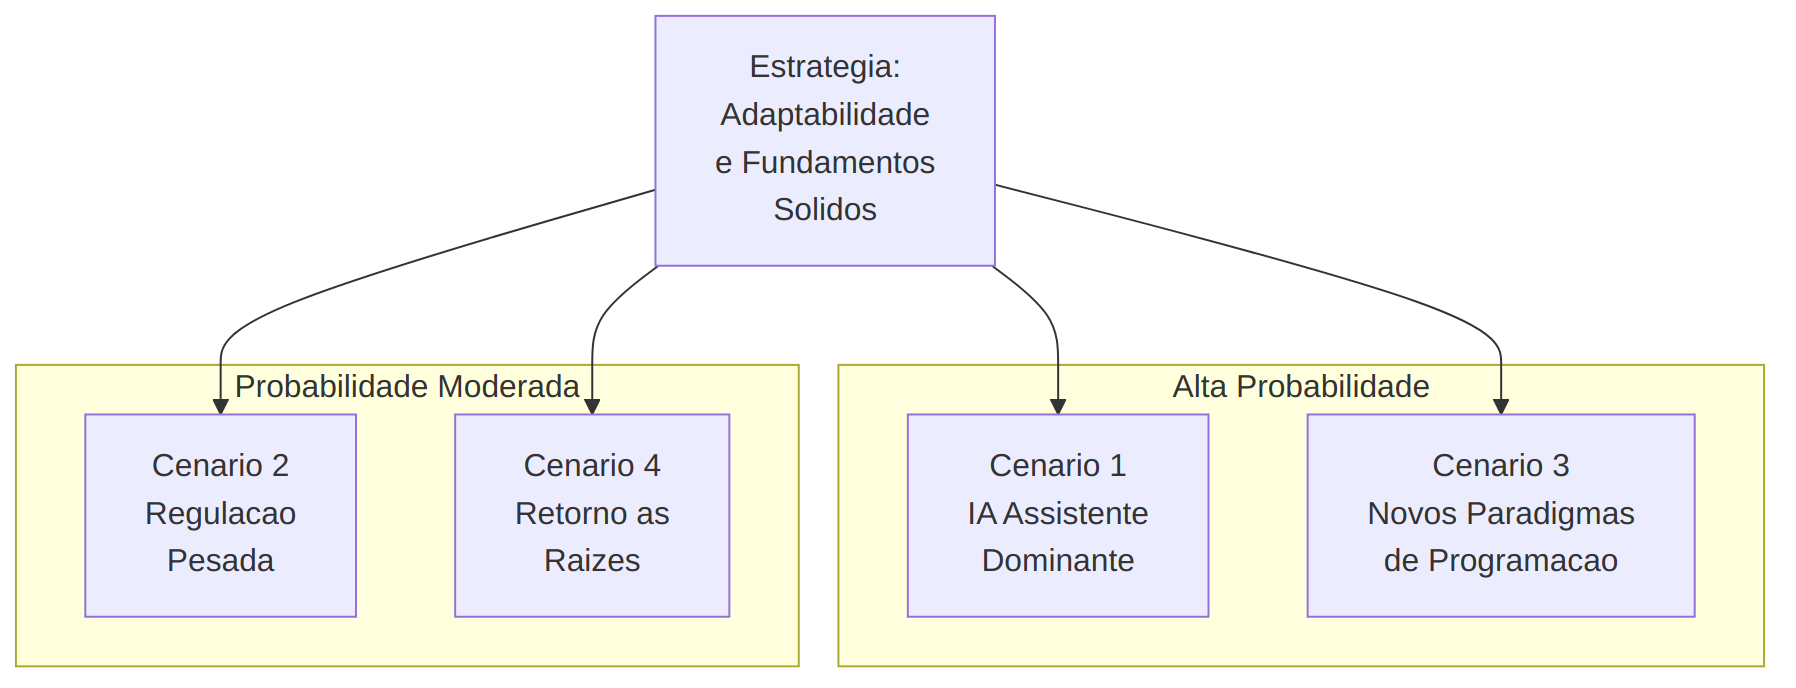
\includegraphics[width=0.85\textwidth]{imagens/12-futuro-engenharia-software-03-quatro-cenarios-para-o-futuro-da-engenharia-de-software.png}
    \caption{Quatro Cenários para o Futuro da Engenharia de Software}
\end{figure}

\section{Princípios Atemporais}

Se há algo que este livro defende, é que princípios duram mais que ferramentas.
Enquanto LLMs, frameworks e metodologias vêm e vão, os princípios a seguir
permanecerão relevantes enquanto software for construído por e para humanos.

\subsection{Pensamento Crítico}

\begin{itemize}
    \item Questionar premissas antes de aceitar requisitos.
    \item Desconfiar de soluções que parecem boas demais.
    \item Distinguir correlação de causalidade, opinião de evidência.
    \item Na era da IA: questionar saídas geradas com o mesmo rigor que se questiona
    código de um colega junior.
\end{itemize}

\subsection{Resolução de Problemas}

\begin{itemize}
    \item Decompor problemas grandes em problemas menores.
    \item Identificar o problema real antes de buscar a solução.
    \item Primeira solução que funciona raramente é a melhor. Iterar.
    \item Saber quando parar de otimizar. ``Bom o suficiente'' é uma decisão
    legítima de engenharia.
\end{itemize}

\subsection{Comunicação e Empatia}

\begin{itemize}
    \item Software é construído por pessoas para pessoas.
    \item Saber explicar decisões técnicas para não-técnicos é superpoder.
    \item Ouvir antes de propor. Entender o contexto antes de sugerir a solução.
    \item Empatia com o usuário: o que parece ``óbvio'' para o engenheiro pode ser
    incompreensível para quem usa.
\end{itemize}

\subsection{Curiosidade Intelectual}

\begin{itemize}
    \item Os melhores engenheiros que conheci compartilham uma característica:
    curiosidade insaciável.
    \item Ler fora da bolha: filosofia, biologia, economia. As melhores analogias
    para software vêm de outros domínios.
    \item Perguntar ``por quê?'' até chegar à raiz. Cinco porquês.
    \item Experimentar tecnologias novas não porque são novas, mas porque expandem
    o repertório.
\end{itemize}

\subsection{Humildade Técnica}

\begin{itemize}
    \item Admitir quando não sabe. ``Não sei, mas vou descobrir'' é a resposta mais
    profissional possível.
    \item O código que você escreveu há 6 meses provavelmente tem problemas.
    Aceite isso com naturalidade.
    \item A melhor solução pode vir do estagiário. Hierarquia não determina qualidade
    de ideias.
    \item Estar disposto a ser convencido por evidências, mesmo quando contrariam
    sua opinião.
\end{itemize}

\subsection{Coragem para Mudar --- e para Não Mudar}

\begin{itemize}
    \item \textbf{Coragem para mudar}: refatorar código legado, questionar decisões
    estabelecidas, propor alternativas quando o status quo não funciona.
    \item \textbf{Coragem para não mudar}: resistir à moda quando o que funciona
    é suficiente. Não migrar para microserviços ``porque todo mundo está
    fazendo''. Não adotar a linguagem nova ``porque é hype''.
    \item \textbf{O equilíbrio}: sabedoria é saber quando aplicar cada coragem.
    Pesa mais a evidência do que a tendência.
\end{itemize}

\subsection{Mentalidade de Crescimento}

\begin{itemize}
    \item \textbf{Growth mindset}: inteligência e habilidade não são fixas. São
    desenvolvidas com esforço, prática e feedback.
    \item \textbf{Erro como aprendizado}: todo bug é uma aula. Toda falha em produção
    é uma melhoria futura. Post-mortems sem culpa.
    \item \textbf{Conforto com desconforto}: aprender coisas novas é desconfortável.
    Esse desconforto é o sinal de que você está crescendo.
    \item \textbf{Comparação consigo mesmo}: o único benchmark que importa é ``eu sou
    melhor do que era há um ano?''
\end{itemize}

\subsection{Pensamento Sistêmico}

Retomamos aqui o conceito do Capítulo 0, agora em perspectiva ampliada.

\begin{itemize}
    \item \textbf{Sistemas dentro de sistemas}: seu código é parte de um serviço, que
    é parte de uma plataforma, que é parte de um negócio, que é parte de um
    ecossistema. Cada nível tem suas dinâmicas.
    \item \textbf{Feedback loops}: ações geram consequências que influenciam ações
    futuras. Entender esses ciclos é entender sistemas complexos.
    \item \textbf{Propriedades emergentes}: o comportamento do sistema inteiro não
    pode ser previsto analisando cada componente isoladamente.
    \item \textbf{O pensamento sistêmico na era da IA}: sistemas com componentes
    de IA são \textit{ainda mais} imprevisíveis. Modelos podem se comportar
    de formas inesperadas em produção. O pensamento sistêmico não é opcional
    --- é sobrevivência.
\end{itemize}

\section{Conclusão Final do Livro}

\subsection{A Jornada Através dos Capítulos}

Ao longo de treze capítulos, percorremos um caminho que começa nos fundamentos e
termina no futuro.

\begin{figure}[htbp]
    \centering
    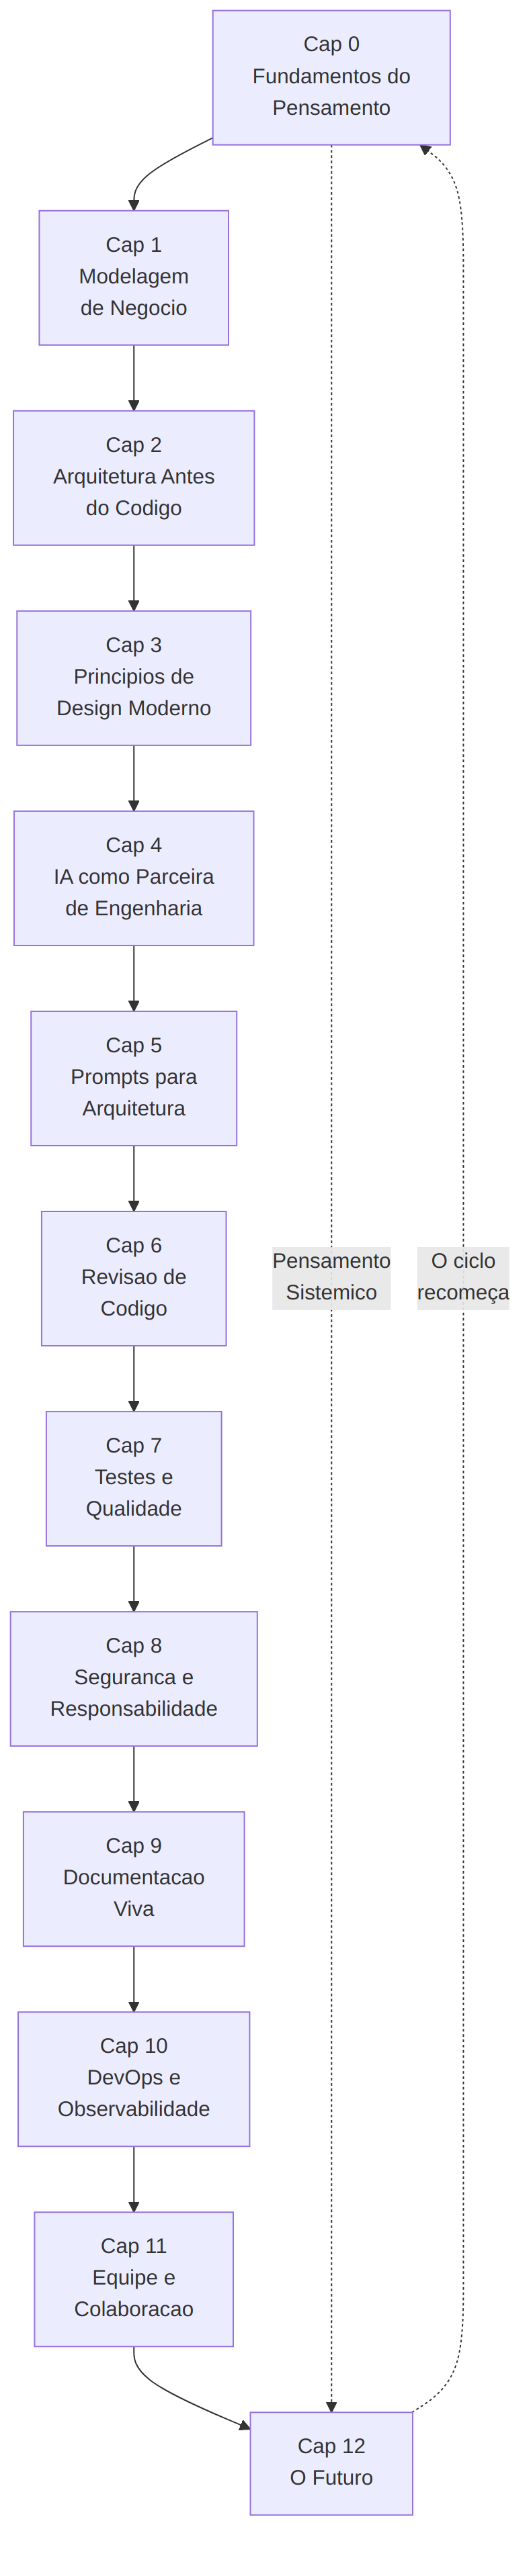
\includegraphics[width=0.85\textwidth]{imagens/12-futuro-engenharia-software-04-mapa-de-conexoes-dos-capitulos-do-livro.png}
    \caption{Mapa de Conexões dos Capítulos do Livro}
\end{figure}

\begin{itemize}
    \item \textbf{Capítulo 0 --- Fundamentos}: estabelecemos que engenharia é, antes de
    tudo, uma forma de pensar. Pensamento sistêmico, trade-offs, ética.
    \item \textbf{Capítulo 1 --- Modelagem de Negócio}: aprendemos a modelar o domínio
    antes de escrever uma linha de código. IDEF-0, RM-ODP.
    \item \textbf{Capítulo 2 --- Arquitetura}: a arquitetura vem antes do código.
    Decisões estruturais definem o sucesso ou fracasso do sistema.
    \item \textbf{Capítulo 3 --- Princípios de Design}: SOLID, KISS, YAGNI, DRY ---
    bússolas que guiam quando o mapa não existe.
    \item \textbf{Capítulo 4 --- IA como Parceira}: aprendemos a colaborar com a IA,
    entendendo suas capacidades e limitações.
    \item \textbf{Capítulo 5 --- Prompts}: a arte e a ciência de se comunicar com
    LLMs para obter resultados de qualidade em arquitetura e código.
    \item \textbf{Capítulo 6 --- Revisão de Código}: o olhar crítico sobre o que é
    produzido, seja por humanos ou por IA.
    \item \textbf{Capítulo 7 --- Testes e Qualidade}: a rede de segurança que
    permite mudar com confiança.
    \item \textbf{Capítulo 8 --- Segurança}: responsabilidade sobre o que construímos
    e como protegemos quem usa.
    \item \textbf{Capítulo 9 --- Documentação Viva}: conhecimento que evolui junto
    com o código, não em documentos esquecidos.
    \item \textbf{Capítulo 10 --- DevOps e Observabilidade}: do código ao deploy,
    do deploy à observação, da observação à melhoria.
    \item \textbf{Capítulo 11 --- Equipe e Colaboração}: software é esporte coletivo.
    Times fortes constroem sistemas fortes.
    \item \textbf{Capítulo 12 --- O Futuro}: este capítulo. O ciclo se fecha e
    recomeça.
\end{itemize}

\subsection{O Pensamento de Engenharia é a Ferramenta Definitiva}

Ferramentas mudam. Linguagens mudam. Frameworks mudam. LLMs mudam. O que não muda
é a capacidade de \textbf{pensar com rigor} sobre o que estamos construindo, para
quem e por quê.

\begin{itemize}
    \item O engenheiro que pensa bem usa qualquer ferramenta bem.
    \item O engenheiro que não pensa produz lixo sofisticado --- com ou sem IA.
    \item Este livro não é sobre código. É sobre o \textbf{pensamento} que antecede,
    acompanha e sucede o código.
\end{itemize}

\subsection{IA é o Meio, Não o Fim}

\begin{itemize}
    \item A IA é a ferramenta mais poderosa que engenheiros de software já tiveram.
    Mas continua sendo \textit{ferramenta}.
    \item O objetivo não é usar IA. O objetivo é construir software que resolve
    problemas reais de forma confiável, segura e sustentável. Se a IA ajuda,
    ótimo. Se atrapalha, descarte-a.
    \item O risco da ``IA como martelo'': quando tudo que você tem é IA, tudo parece
    um prompt.
    \item A maturidade é saber quando usar IA, quando não usar, e quando usar
    parcialmente.
\end{itemize}

\subsection{Chamado à Ação: Pense, Não Apenas Codifique}

\begin{itemize}
    \item Antes de abrir o editor, abra o caderno. Desenhe. Questione. Modele.
    \item Antes de gerar código com IA, entenda o que precisa ser gerado e por quê.
    \item Antes de aceitar o output de um agente, valide se ele resolve o problema
    certo da forma certa.
    \item Antes de seguir a tendência, pergunte: ``Isso resolve um problema real
    que eu tenho?''
    \item Antes de otimizar, meça. Antes de medir, defina o que importa.
\end{itemize}

\subsection{O Futuro Pertence aos que Pensam Sobre o que Constroem}

\vspace{0.5cm}

Existe uma tentação, na era da IA, de acreditar que o pensamento se tornou
obsoleto. Que a velocidade substituiu a reflexão. Que gerar é mais importante
que entender.

O oposto é verdadeiro.

Quanto mais poderosas são nossas ferramentas, mais importante é a sabedoria
de quem as dirige. Um bisturi na mão de um cirurgião salva vidas. O mesmo
bisturi, sem conhecimento e julgamento, é apenas uma lâmina perigosa.

Nós, engenheiros de software, construímos o tecido digital da civilização.
Os sistemas que projetamos determinam como pessoas se comunicam, como empresas
operam, como governos servem cidadãos, como o conhecimento é preservado e
transmitido. Essa é uma responsabilidade que nenhuma IA pode assumir por nós.

O futuro da engenharia de software não será definido por qual modelo de linguagem
é mais avançado, nem por qual framework é mais popular, nem por qual empresa
levanta mais capital. Será definido pela \textbf{qualidade do pensamento} que
colocamos em cada decisão, cada arquitetura, cada linha de código --- seja ela
escrita por nós ou por uma máquina que supervisionamos.

\textit{Pense bem. Construa com propósito. Questione sempre. Aprenda para sempre.}

\textit{O futuro pertence a quem pensa sobre o que constrói.}

\section*{Exercícios Finais}

Estes exercícios são reflexivos. Não há resposta certa. O valor está no
processo de pensar.

\begin{enumerate}
    \item \textbf{Visão pessoal}: Escreva um texto de uma página descrevendo como
    você se vê como engenheiro(a) de software daqui a 5 anos. Que tipo de
    problemas quer resolver? Que habilidades quer ter? Que impacto quer causar?

    \item \textbf{Plano de desenvolvimento}: Identifique 3 habilidades que este livro
    revelou como importantes e que você ainda não domina. Para cada uma, defina:
    (a) por que é importante para você, (b) como vai aprender, (c) como vai
    medir progresso.

    \item \textbf{Princípio pessoal}: Escolha o princípio de engenharia que mais
    ressoou com você ao longo do livro. Escreva por que ele é importante e
    como você pretende aplicá-lo no seu trabalho diário.

    \item \textbf{Análise de cenário}: Escolha um dos 4 cenários futuros apresentados
    neste capítulo. Descreva como ele impactaria sua carreira atual e que
    ações você tomaria para se adaptar.

    \item \textbf{Carta ao eu do futuro}: Escreva uma carta para você mesmo(a), a
    ser lida em 2030. Descreva suas expectativas, seus medos, suas esperanças
    sobre o futuro da engenharia de software. Guarde essa carta.

    \item \textbf{Exercício de ensino}: Escolha um conceito de qualquer capítulo
    deste livro. Explique-o para alguém que não é da área de tecnologia, em
    no máximo 5 minutos. O que funcionou? O que foi difícil de explicar?

    \item \textbf{Auditoria de IA}: Na próxima semana, registre toda vez que usar
    IA no seu trabalho. Para cada uso, anote: (a) a tarefa, (b) o resultado,
    (c) se você validou o resultado, (d) se a IA agregou valor real.
    Ao final, analise os padrões.

    \item \textbf{Design de sistema com restrições}: Projete (apenas no papel) um
    sistema de software que não pode usar IA em nenhuma parte do seu
    desenvolvimento ou operação. Que desafios isso apresenta? O que ficou mais
    difícil? O que ficou mais fácil?
\end{enumerate}

\section*{Leituras Recomendadas}

\begin{table}[h]
\centering
\caption{Leituras Recomendadas por Tema}
\begin{tabular}{p{3.5cm} p{8cm}}
\toprule
\textbf{Tema} & \textbf{Obras Recomendadas} \\
\midrule
Arquitetura de Software &
    \textit{Clean Architecture} --- Robert C. Martin \newline
    \textit{Fundamentals of Software Architecture} --- Richards \& Ford \newline
    \textit{Building Evolutionary Architectures} --- Ford, Parsons \& Kua \newline
    \textit{Software Architecture: The Hard Parts} --- Ford et al. \\
\midrule
Domain-Driven Design &
    \textit{Domain-Driven Design} --- Eric Evans \newline
    \textit{Implementing DDD} --- Vaughn Vernon \newline
    \textit{Learning Domain-Driven Design} --- Vlad Khononov \\
\midrule
Engenharia e Práticas &
    \textit{The Pragmatic Programmer} --- Hunt \& Thomas \newline
    \textit{A Philosophy of Software Design} --- John Ousterhout \newline
    \textit{Refactoring} --- Martin Fowler \newline
    \textit{Working Effectively with Legacy Code} --- Michael Feathers \\
\midrule
DevOps e Entrega &
    \textit{Accelerate} --- Forsgren, Humble \& Kim \newline
    \textit{The Phoenix Project} --- Kim, Behr \& Spafford \newline
    \textit{Continuous Delivery} --- Humble \& Farley \newline
    \textit{Site Reliability Engineering} --- Google \\
\midrule
Equipes e Organizações &
    \textit{Team Topologies} --- Skelton \& Pais \newline
    \textit{An Elegant Puzzle} --- Will Larson \newline
    \textit{Staff Engineer} --- Will Larson \newline
    \textit{The Manager's Path} --- Camille Fournier \\
\midrule
IA e Futuro &
    \textit{AI Engineering} --- Chip Huyen \newline
    \textit{Designing Machine Learning Systems} --- Chip Huyen \newline
    \textit{The Alignment Problem} --- Brian Christian \newline
    \textit{Atlas of AI} --- Kate Crawford \\
\midrule
Pensamento e Carreira &
    \textit{Thinking in Systems} --- Donella Meadows \newline
    \textit{The Fifth Discipline} --- Peter Senge \newline
    \textit{Antifragile} --- Nassim Taleb \newline
    \textit{Range} --- David Epstein \\
\bottomrule
\end{tabular}
\end{table}

\subsection*{Papers e Artigos Fundamentais}

\begin{itemize}
    \item \textit{No Silver Bullet} --- Fred Brooks (1987). Por que não existe
    solução mágica em engenharia de software. Tão relevante hoje quanto há
    quase 40 anos.
    \item \textit{Out of the Tar Pit} --- Moseley \& Marks (2006). Complexidade
    como o principal inimigo do software.
    \item \textit{Attention Is All You Need} --- Vaswani et al. (2017). O paper que
    originou a arquitetura Transformer, base de todos os LLMs modernos.
    \item \textit{On the Measure of Intelligence} --- François Chollet (2019).
    Uma proposta para medir inteligência de forma independente do domínio.
    \item \textit{DORA State of DevOps Reports} (anual). Dados sobre práticas de
    engenharia que realmente impactam performance organizacional.
\end{itemize}

\subsection*{Blogs e Newsletters}

\begin{itemize}
    \item \textbf{Martin Fowler Blog} (\texttt{martinfowler.com}): referência em
    arquitetura e design de software.
    \item \textbf{The Pragmatic Engineer} (Gergely Orosz): newsletter sobre engenharia
    de software em empresas de tecnologia.
    \item \textbf{ByteByteGo} (Alex Xu): system design explicado visualmente.
    \item \textbf{Simon Willison Blog} (\texttt{simonwillison.net}): cobertura
    excelente de IA aplicada a desenvolvimento.
    \item \textbf{Lenny's Newsletter}: produto e tecnologia na interseção com negócios.
    \item \textbf{Staff Eng} (\texttt{staffeng.com}): histórias e guias para
    carreiras técnicas avançadas.
\end{itemize}

\subsection*{Comunidades e Conferências}

\begin{itemize}
    \item \textbf{QCon}: conferência voltada para engenheiros seniores e arquitetos.
    \item \textbf{GOTO Conference}: palestras práticas sobre engenharia moderna.
    \item \textbf{The DEVOPS Conference}: foco em cultura DevOps e plataformas.
    \item \textbf{PyCon, JSConf, RustConf}: conferências por linguagem, com forte
    componente de comunidade.
    \item \textbf{Meetups locais}: comunidades em São Paulo, Rio, Belo Horizonte,
    Recife, Florianópolis e outras cidades brasileiras com cenas tech ativas.
    \item \textbf{Comunidades online}: Dev.to, Hacker News, Reddit (r/programming,
    r/ExperiencedDevs), Discord de projetos open source.
\end{itemize}

\section*{Glossário}

\begin{longtable}{p{3.5cm} p{8.5cm}}
\caption{Glossário de Termos} \\
\toprule
\textbf{Termo} & \textbf{Definição} \\
\midrule
\endfirsthead
\toprule
\textbf{Termo} & \textbf{Definição} \\
\midrule
\endhead
\midrule
\multicolumn{2}{r}{\textit{Continua na próxima página...}} \\
\bottomrule
\endfoot
\bottomrule
\endlastfoot

ADR (Architecture Decision Record) &
    Documento que registra uma decisão de arquitetura, seu contexto, as
    alternativas consideradas e as consequências. Cria um histórico
    rastreável de decisões técnicas. \\
\midrule
Agent (Agente de IA) &
    Sistema de IA capaz de executar ações autônomas em um ambiente, como
    navegar repositórios, executar comandos e iterar sobre resultados.
    Diferente de um chatbot, o agente \textit{age}, não apenas responde. \\
\midrule
API (Application Programming Interface) &
    Conjunto de definições e protocolos que permite a comunicação entre
    componentes de software. Define como sistemas se conectam e trocam
    dados. \\
\midrule
CI/CD (Continuous Integration / Continuous Delivery) &
    Prática de integrar código frequentemente (CI) e manter o software
    sempre em estado implantável (CD). Automatiza build, testes e deploy. \\
\midrule
Clean Architecture &
    Padrão arquitetural proposto por Robert C. Martin em que as dependências
    apontam para o centro (domínio), isolando regras de negócio de
    frameworks e infraestrutura. \\
\midrule
Cloud Native &
    Abordagem de construção de software projetada desde o início para
    aproveitar a elasticidade, resiliência e automação de ambientes de
    nuvem. \\
\midrule
Context Window &
    A quantidade máxima de texto (medida em tokens) que um LLM consegue
    processar em uma única interação. Limita quanto contexto o modelo
    ``vê'' de uma vez. \\
\midrule
DDD (Domain-Driven Design) &
    Abordagem de design de software que coloca o domínio de negócio no
    centro das decisões. Conceitos-chave: Bounded Context, Aggregate,
    Entity, Value Object, Ubiquitous Language. \\
\midrule
Deploy &
    Processo de disponibilizar uma versão de software em um ambiente (staging,
    produção). Pode ser manual ou automatizado via pipeline de CI/CD. \\
\midrule
DevOps &
    Cultura e conjunto de práticas que unifica desenvolvimento (Dev) e
    operações (Ops), promovendo colaboração, automação e feedback rápido. \\
\midrule
Dívida Técnica &
    Atalhos e decisões subótimas no código que facilitam a entrega presente
    mas aumentam o custo de manutenção futura. Como dívida financeira:
    acumula juros. \\
\midrule
Feature Flag &
    Mecanismo que permite habilitar ou desabilitar funcionalidades em
    produção sem deploy. Usado para releases graduais, testes A/B e
    rollback rápido. \\
\midrule
Hallucination (Alucinação) &
    Quando um LLM gera informação que parece plausível mas é factualmente
    incorreta: bibliotecas que não existem, APIs inventadas, código que
    não compila. \\
\midrule
IaC (Infrastructure as Code) &
    Prática de gerenciar e provisionar infraestrutura através de arquivos
    de configuração versionados (Terraform, Pulumi, CloudFormation),
    em vez de processos manuais. \\
\midrule
IDEF-0 &
    Método de modelagem funcional que representa processos como atividades
    com entradas, saídas, controles e mecanismos. Útil para entender
    sistemas antes de implementá-los. \\
\midrule
LLM (Large Language Model) &
    Modelo de inteligência artificial treinado em grandes volumes de texto,
    capaz de gerar e compreender linguagem natural e código. Exemplos:
    GPT-4, Claude, Gemini, LLaMA. \\
\midrule
Microsserviço &
    Estilo arquitetural onde o sistema é composto por serviços pequenos,
    independentes e implantáveis separadamente, cada um responsável por
    uma capacidade de negócio. \\
\midrule
Monolito &
    Arquitetura onde toda a aplicação é uma única unidade implantável.
    Não é inerentemente ruim --- é simples, e frequentemente a escolha
    correta para sistemas menores. \\
\midrule
Observabilidade &
    Capacidade de entender o estado interno de um sistema a partir de
    suas saídas externas. Três pilares: logs, métricas e traces
    distribuídos. \\
\midrule
Prompt Engineering &
    A prática de formular instruções e contexto para modelos de IA de
    forma a obter os melhores resultados possíveis. Combina clareza,
    especificidade e estrutura. \\
\midrule
RAG (Retrieval-Augmented Generation) &
    Técnica que combina busca em bases de dados com geração por LLM.
    O modelo consulta documentos relevantes antes de gerar uma resposta,
    reduzindo alucinações. \\
\midrule
Refactoring &
    Reestruturação de código existente sem alterar seu comportamento
    externo. Objetivo: melhorar legibilidade, manutenibilidade e design
    interno. \\
\midrule
RM-ODP (Reference Model for Open Distributed Processing) &
    Framework de modelagem que organiza a visão de um sistema em cinco
    viewpoints: empresa, informação, computação, engenharia e tecnologia. \\
\midrule
SLA (Service Level Agreement) &
    Acordo formal entre provedor e cliente sobre o nível de serviço
    esperado. Define métricas, limites e consequências de descumprimento. \\
\midrule
SLI (Service Level Indicator) &
    Métrica quantitativa que mede um aspecto do nível de serviço. Exemplo:
    latência do percentil 99, taxa de erros, disponibilidade. \\
\midrule
SLO (Service Level Objective) &
    Meta interna para um SLI. Exemplo: ``99.9\% das requisições devem
    ter latência abaixo de 300ms''. Mais restritivo que o SLA. \\
\midrule
SOLID &
    Cinco princípios de design orientado a objetos: Single Responsibility,
    Open/Closed, Liskov Substitution, Interface Segregation, Dependency
    Inversion. \\
\midrule
SRE (Site Reliability Engineering) &
    Disciplina que aplica princípios de engenharia de software a operações
    de infraestrutura. Foco em automação, error budgets e confiabilidade
    como feature. \\
\midrule
TDD (Test-Driven Development) &
    Prática de escrever o teste antes do código de produção. Ciclo:
    Red (teste falha) $\rightarrow$ Green (código passa) $\rightarrow$
    Refactor (melhoria). \\
\midrule
Token &
    Unidade de processamento de texto em LLMs. Aproximadamente 3/4 de
    uma palavra em inglês. Modelos têm limites de tokens por interação
    (context window) e por geração. \\
\midrule
Trade-off &
    Decisão que envolve trocar um benefício por outro. Em engenharia:
    performance vs. legibilidade, velocidade vs. qualidade, simplicidade
    vs. flexibilidade. Não há almoço grátis. \\
\midrule
Twelve-Factor App &
    Metodologia para construção de aplicações SaaS modernas, definindo
    12 práticas como config por variáveis de ambiente, statelessness e
    logs como streams de eventos. \\
\midrule
Ubiquitous Language &
    Linguagem compartilhada entre desenvolvedores e especialistas de
    domínio em DDD. Os mesmos termos no código, na documentação e nas
    conversas. Elimina tradução e ambiguidade. \\

\end{longtable}

\begin{figure}[htbp]
    \centering
    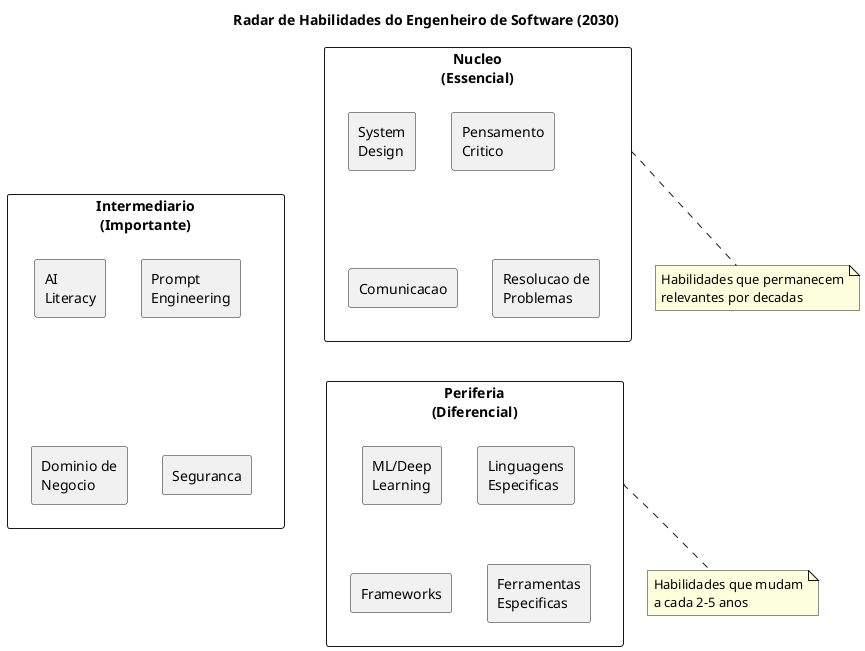
\includegraphics[width=0.85\textwidth]{imagens/12-futuro-engenharia-software-05-radar-de-habilidades-futuras-do-engenheiro-de-software.png}
    \caption{Radar de Habilidades Futuras do Engenheiro de Software}
\end{figure}

\vspace{1cm}

\begin{center}
\large\textit{``O futuro pertence àqueles que acreditam na beleza dos seus sonhos.''\\
--- Eleanor Roosevelt}

\vspace{0.5cm}

\normalsize E, para engenheiros de software, àqueles que pensam com cuidado sobre o que constroem.

\vspace{1cm}

\textbf{--- FIM ---}
\end{center}
